
\chapter{Introduction to Nonlinear Waves}\label{chap1}

\section{One dimensional linear equation}\pageoriginale\label{chap1:sec1.1}

The Wave equation
$$
\phi_{tt}=c_0^2 \nabla^2\phi
$$
occurs in the classical fields of acoustics, electromagnetism and elasticity and many familiar ``mathematical methods'' were developed on it. 

The solution of the one-demensional form,
\begin{equation}
\phi_{tt}-c_0^2\phi_{xx}=0,\tag{1.1}\label{chap1:eq1.1}
\end{equation}
is almost trivial. Introducing the variables $\alpha,\beta$ by 
\begin{align*}
\alpha &= x-c_0t,\\
\beta &= x+c_0t,
\end{align*}
equation \eqref{chap1:eq1.1} becomes $\phi_{\alpha\beta}=0$. The general solution of this equation is 
$$
\phi=f(\alpha)+g(\beta)
$$

Therefore, the general solution of \eqref{chap1:eq1.1} is 
\begin{equation}
\phi(x,t)=f(x-c_0t)+g(x+c_0t);\tag{1.2}\label{chap1:eq1.2}
\end{equation}
$f,g$ are determined by the initial or boundary conditions.
\begin{itemize}
\item [(i)] For the initial value problem
$$
t=0:\phi=\phi_0(x), \phi_t=\phi_1(x)>-\infty <x<\infty,
$$
the solution is 
\begin{equation}
\phi(x,t)=\frac{\phi_0(x-c_0t)+\phi_0(x+c_0t)}{2}+\frac{1}{2c_0}\int\limits_{x-c_0t}^{x+c_0t}\phi_1(s)\,ds.\tag{1.3}\label{chap1:eq1.3}
\end{equation}\pageoriginale
\item [(ii)] For the signalling problem 
\begin{align*}
t &=0:\phi=0,\phi_t=0,x>0,\\
x&=0:\phi=\phi(t),t>0,
\end{align*}
the solution in $x>0,t>0$, is 
\begin{equation}
\phi=
\begin{cases}
0 & , t<\frac{x}{c_0},\\
\phi\left(t-\frac{x}{c_0}\right) &, t>\frac{x}{c_0}. \tag{1.4}\label{chap1:eq1.4}
\end{cases}
\end{equation}
\end{itemize}

\section{A basic non-linear wave equation}\label{chap1:sec1.2}

The solution $f$ and $g$ correspond to the two factors when equation \eqref{chap1:eq1.1} is written as 
$$
\left(\frac{\partial}{\partial t}+c_0\frac{\partial}{\partial t}\right)\quad \left(\frac{\partial}{\partial t}-c_0\frac{\partial}{\partial x}\right)\phi=0.
$$

While equation \eqref{chap1:eq1.1} is simple to handle it would be given simpler if only one of the factors occurred, and we had, for example,
$$
\frac{\partial\phi}{\partial t}+c_0\frac{\partial\phi}{\partial x}=0,
$$
with the solution $\phi=f(x-c_0 t)$. 

The simplest non-linear wave equation is a counterpart of this,\break
namely: 
\begin{equation}
\frac{\partial\phi}{\partial t}+c(\phi)\frac{\partial\phi}{\partial
  x}=0, t>0, -\infty <x < \infty,\tag{1.5}\label{chap1:eq1.5} 
\end{equation}
where $c(\phi)$ is a given function of $\phi$. For the initial value
problem, we would add the initial condition 
\begin{equation}
t=0:\phi=f(x),\, -\infty <x<\infty.\tag{1.6}\label{chap1:eq1.6}
\end{equation}\pageoriginale

Though this equation looks simple it poses nontrivial problems in the
analysis and leads to new phenomena. 

The equation can be solved by the method of characteristics. The idea
is to note that a linear combination 
\begin{equation}
a\frac{\partial\phi}{\partial t}+b\frac{\partial\phi}{\partial x} \tag{1.7}\label{chap1:eq1.7}
\end{equation}
can be interpreted as the directional derivative of $\phi$ in the direction $(a,b)$. A characteristic curve is introduced such that its direction is $(a,b)$ at each point. Then the equation provides information on the rate of change of $\phi$ on this curve and we have effectively an ordinary differential equation, which leads to the solution. In applying this idea and carrying out the details for \eqref{chap1:eq1.5}, we first consider any curve $
\mathscr{C}$ described by $x=x(t)$. (See Fig.~\ref{chap1:fig1.1})
\begin{figure}[H]
\centering
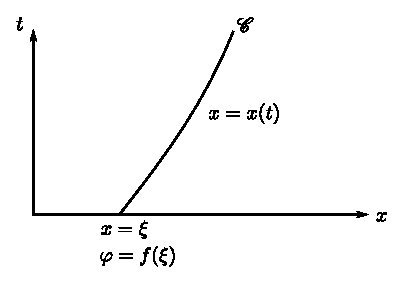
\includegraphics{figures/fig61-1.1.eps}
\caption{}
\label{chap1:fig1.1}
\end{figure}

On $\mathscr{C}$, we have 
$$
\phi=\phi(x(t),t);
$$
\ie $\phi$ may be treated temporarily as a function of $t$. Furthermore, on $\mathscr{c}$ we have 
\begin{equation}
\frac{d\phi}{dt}=\phi_t+\frac{dx}{dt}\phi_x\tag{1.8}\label{chap1:eq1.8}
\end{equation}\pageoriginale

Now to implement the idea noted above we choose $\mathscr{C}$ so that $dx/dt=c(\phi)$. Then the right hand side of \eqref{chap1:eq1.8} is just the combination that appears in the equation \eqref{chap1:eq1.5} and we have $d\phi/dt=0$. If the initial point on the characteristic curve is denoted by $\xi$, then the initial condition \eqref{chap1:eq1.6} requires $\phi(0)=f(\xi)$. Combining these we have the following ``characteristic form''.
\setcounter{equation}{8}
\begin{numcases}
{\text{On}\quad \mathscr{C}:}
\frac{dx}{dt}=c(\phi), \quad x(0)=\xi,\label{chap1:eq1.9}\\
\frac{d\phi}{dt}=0, \quad \phi(0)=f(\xi).\label{chap1:eq1.10}
\end{numcases}


We cannot solve \eqref{chap1:eq1.9} independently of \eqref{chap1:eq1.10} since $c$ is a function of $\phi$. Hence we have a coupled pair of ordinary differential equations on $\mathscr{C}$. The solution for $\phi$ depends on theb initial condition; therefore, $\mathscr{C}$ also depends on the initial condition.

Although \eqref{chap1:eq1.9} cannot be solved immediately, \eqref{chap1:eq1.10} can. It gives 
\begin{align*}
\phi &= \text{constant on}\quad\mathscr{C},\\
\intertext{and therefore}
\phi &= f(\xi)\text{ on the whole of}\quad\mathscr{C}.
\end{align*}

Then, returning to \eqref{chap1:eq1.9} and defining $F(\xi)$ by 
$$
F(\xi)=c(f(\xi)),
$$
we\pageoriginale have 
\setcounter{equation}{10}
\begin{equation}
\begin{split}\label{chap1:eq1.11}
\frac{dx}{dt}=F(\xi),\\
x(0)=\xi.
\end{split}
\end{equation}

Integrating \eqref{chap1:eq1.11} we obtain
$$
x=tF(\xi)+\xi.
$$

The characteristic curve is a straight line whose slope depends on
$\xi$. Combining the results we have the solution in parametric form 
\begin{align}
\phi &= f(\xi)\tag{1.12}\label{chap1:eq1.12}\\
x&= \xi +tF(\xi).\tag{1.13}\label{chap1:eq1.13}
\end{align}

In making this construction it is easiest to think of just one particular characteristic curve. But from the final answer \eqref{chap1:eq1.12}-\eqref{chap1:eq1.13}, we can then find the solution in a whole $(x,t)$ region by varying $\xi$. This leads to a change of emphasis: To find $\phi$ at a given $(x,t)$, solve \eqref{chap1:eq1.13} for $\xi(x,t)$ and substitute in \eqref{chap1:eq1.12}. This final form is an analytic statement free of the geometrical construction. We check directly that it solves the problem.

In solving \eqref{chap1:eq1.13}, there is a unique solution $\xi(x,t)$ provided
\begin{equation}
1+tF'(\xi)\neq 0,\tag{1.14}\label{chap1:eq1.14}
\end{equation}
which we assume for the present.

\medskip\noindent
{\bf\large Initial\pageoriginale condition}. When $t=0, \xi=x$ by \eqref{chap1:eq1.13}. Hence \eqref{chap1:eq1.12} implies $\phi=f(x)$.

\medskip\noindent
{\bf\large Equation}. Differentiating the equations \eqref{chap1:eq1.13} and \eqref{chap1:eq1.12} partially w.r.t. $t$ we obtain
\begin{align*}
0&=F(\xi)+\left\{tF'(\xi)+1\right\}\xi_t,\\
\phi_t&= f'(\xi)\xi_t.
\end{align*}

Eliminating $\xi_t$ we have 
$$
\phi_t=-\frac{f'(\xi)F(\xi)}{1+tF'(\xi)}.
$$

Similarly, differentiating the equations \eqref{chap1:eq1.13} and \eqref{chap1:eq1.12} partially w.r.t. $x$ and eliminating $\xi_x$ we find
$$
\phi_x=\frac{f'(\xi)}{1+tF'(\xi)}.
$$

Hence
\begin{align*}
\phi_t + c_{\cdotp} (\phi)\phi_x & = - \frac{f'(\xi)F(\xi)} {1+tF'(\xi)} +F(\xi) \frac{f'(\xi)}{1+tF'(\xi)}\\
& = 0.
\end{align*}

\medskip\noindent
{\bf \large Uniqueness}. If $\psi(x,t)$ is some other solution of \eqref{chap1:eq1.5} and \eqref{chap1:eq1.6} then on $x=\xi +tF(\xi)$
$$
\psi(x,t)=\psi(\xi,0)=f(\xi)=\phi(x,t).
$$

Hence $\psi \equiv\phi$.

Thus we have proved the following.

\begin{theorem*}
The initial value problem
$$
\phi_t+c(\phi)\phi_x=0, t>0, -\infty <x<\infty,
$$
with $t=0:\phi=f(x),\, -\infty < x < \infty$, has a unique solution in 
\begin{equation*}
0<t<\frac{1}{\underset{F'(\xi)<0}{\max}|F'(\xi)|}
\end{equation*}\pageoriginale
if $f\in C^1(\mathbb{R}), c\in C^1(\mathbb{R})$, where 
$$
F(\xi)=c(f(\xi)).
$$

The solution is given in the parametric form:
\begin{align*}
x=\xi +tF(\xi),\\
\phi(x,t)=f(\xi).
\end{align*}
\end{theorem*}

\begin{remark*}
When $c(\phi)=c_0$, a positive constant, equation \eqref{chap1:eq1.5} becomes the linear wave equation:
$$
\phi_t+c_0\phi_x=0.
$$

The characteristic curves are $x=c_0t+\xi$, and $\phi$ is given by 
$$
\phi(x,t)=f(\xi)=f(x-c_0t).
$$
\end{remark*}

\section{Expansion wave}.\label{chap1:sec1.3}

Consider the problem
\begin{align*}
&\phi_t+c(\phi)\phi_x=0,\quad\text{on}\quad t>0, -\infty < x < \infty,\\
& t=0:\phi =f(x), -\infty < x< \infty,
\end{align*}
where
\begin{equation*}
f(x)=
\begin{cases}
\phi_2, \quad\text{if}\quad x\leq 0\\
\text{monotonic increasing, if}\quad 0\leq x\leq L\\
\phi_1,\quad=\text{if}\quad x\geq L,
\end{cases}
\end{equation*}
with $\phi_1>\phi_2$ and $c'(\phi)>0$.

We shall let $c_1=c(\phi_1), c_2=c(\phi_2)$.
\begin{figure}[H]
\centering
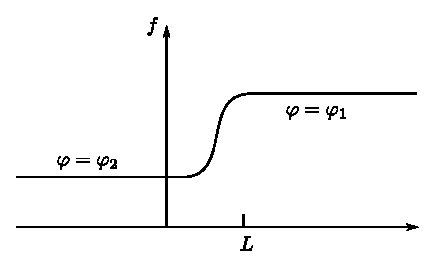
\includegraphics{figures/fig61-1.2.eps}
\caption{}
\label{chap1:fig1.2}
\end{figure}\pageoriginale

We recall the solution of the problem:
\begin{align*}
\phi &= f(\xi),\\
x&=\xi + tF(\xi),\\
\intertext{where}
F(\xi) &= c(f(\xi)).
\end{align*}

Let us consider the characteristics of this problem. For, $\xi\leq 0$,
$$
F(\xi)=c(f(\xi))=c(\phi_2)=c_2.
$$

Therefore, the characteristics through $\xi(\leq 0)$ are straight lines with constant slope $\frac{1}{c_2}$.

For $\xi\geq L, F(\xi)=c(f(\xi))=c(\phi_1)=c_1$. Hence, the characteristics through $\xi(\geq L)$ are also straight lines, with constant slope $\frac{1}{c_1}$. For $0\leq\xi\leq L$, the characteristics through $\xi$ are straight lines having slopes $\frac{1}{F(\xi)}$ with $\frac{1}{c_1}\leq \frac{1}{F(\xi)}\leqq\frac{1}{c_2}$.

Since the characteristics do not intersect, (and this corresponds\break
\eqref{chap1:eq1.14} we obtain $\phi$ as a single valued
function. A\pageoriginale typical $(x,t)$ diagram is shown in
Fig. 1.4(b). 

The behavior of the solution can be explained geometrically as\break shown
in the figures \ref{chap1:fig1.3a}(a), \ref{chap1:fig1.3b}(b). 
\begin{center}
\begin{minipage}[b]{5cm}
\begin{figure}[H]
\centering
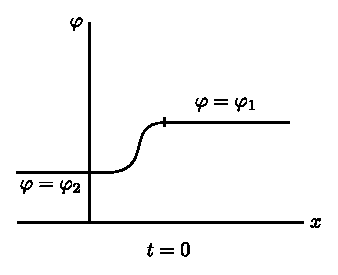
\includegraphics[scale=.9]{figures/fig61-1.3a.eps}
\caption{(a)}
\label{chap1:fig1.3a}
\end{figure}
\end{minipage}
\qquad
\begin{minipage}[b]{5cm}
\setcounter{figure}{2}
\begin{figure}[H]
\centering
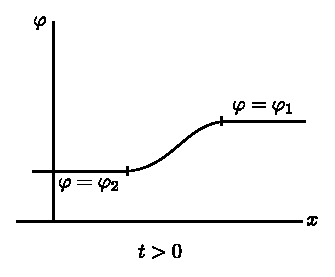
\includegraphics[scale=.9]{figures/fig61-1.3b.eps}
\caption{(b)}
\label{chap1:fig1.3b}
\end{figure}
\end{minipage}
\end{center}

Every point $(\xi,\phi(\xi))$ at $t=0$ will move parallel to the
$x$-axis through a distance $ct_1$ in time $t_1$. Since
$c'(\phi)>0,\phi_2<\phi_1$, the points $(\xi,\phi_1)(\xi\geq L)$
move faster than the points $(\xi,\phi_2)\quad(\xi\leq 0)$. Hence, the
graph of $\phi$ at $t=0$ is stretched as the time increases. 

The analytic details can be carried out most easily by working
entirely with $c$ as the dependent variable. 
\medskip

\noindent {\bf \large Equation for $C$:}

Consider the equation
\begin{align*}
&\phi_t+c(\phi)\phi_x=0\quad\text{in}\quad t>0,\, -\infty < x < \infty\\
& t=0: \phi=f(x), \, -\infty < x < \infty.
\end{align*}

We have found that $c(\phi)$ is the ``propagation speed'', and in constructing solutions we have to deal with two functions, namely, $\phi$ and $c$. But by multiplying the equation by $c'(\phi)$ we obtain
\begin{equation}
\left.
\begin{aligned}
C_t+CC_x &= 0\quad\text{in}\quad t>0, -\infty < x < \infty,\\
t=0: C&= F(x), -\infty < x < \infty,
\end{aligned}
\right\}\tag{1.15}\label{chap1:eq1.15}
\end{equation}\pageoriginale
where $C(x,t)=c(\phi(x,t))$ and
$$
F(\xi)=c(f(\xi)).
$$

This equation involves only the unknown function
$C(x,t)=c\break(\phi(x,t))$; we can recover $\phi$ from $C$ afterwards. The
solution of the problem in \eqref{chap1:eq1.15} is  
\begin{equation}
\begin{aligned}
x &=\xi +tF(\xi),\\
C &= F(\xi),
\end{aligned}\tag{1.16}\label{chap1:eq1.16}
\end{equation}
In the special case,
\begin{equation*}
C(x,0)=
\begin{cases}
c_2\quad\text{in}\quad x\leq 0,\\
c_2 +\frac{c_1-c_2}{L}x\quad\text{in}\quad 0\leq x\leq L,\\
c_1\quad\text{in}\quad x\geq L,
\end{cases}
\end{equation*}
the $x-t$ diagram is shown below in Fig. 1.4(b).
\begin{center}
\begin{minipage}[b]{5cm}
\begin{figure}[H]
\centering
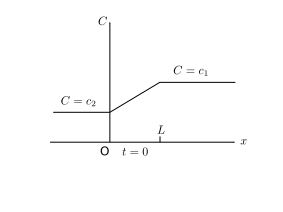
\includegraphics[scale=.8]{figures/fig61-1.4a.eps}
\caption{(a)}
\label{chap1:fig1.4a}
\end{figure}
\end{minipage}
\qquad
\begin{minipage}[b]{5cm}
\setcounter{figure}{3}
\begin{figure}[H]
\centering
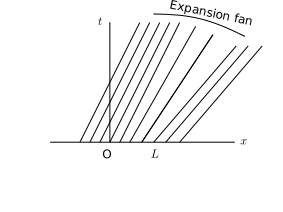
\includegraphics[scale=.8]{figures/fig61-1.4b.eps}
\caption{(b)}
\label{chap1:fig1.4b}
\end{figure}
\end{minipage}
\end{center}

\section{Centred expansion wave}\label{chap1:sec1.4}

We now consider the limiting case of the above problem, as $L\to 0$. In the limit the interval $[c_2,c_1]$ is associated with\pageoriginale the origin. In the limit we will have the characteristics
\begin{align*}
x&=\xi+t c_2,\quad\text{if}\quad \xi<0,\\
x&=\xi+t c_1,\quad\text{if}\quad \xi>0,\\
x&=Ct,\quad\text{if}\quad \xi=0, c_2\leq C\leq c_1.
\end{align*}

The collection of characteristics $x=Ct:C\in[c_2, c_1]$ through the origin is called a `Centred fan' and we have $C=x/t$. In this case the full solution is 
\begin{equation}
C=
\begin{cases}
c_2,\quad\text{if}\quad x \leq c_2 t,\\
x/t,\quad\text{if}\quad c_2 t<x< c_1 t\\
c_1,\quad\text{if}\quad x\geq c_1 t.
\end{cases}\tag{1.17}\label{chap1:eq1.17}
\end{equation}

\begin{center}
\begin{minipage}[t]{5cm}
\begin{figure}[H]
\centering
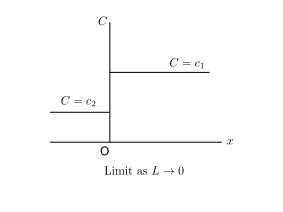
\includegraphics[scale=.9]{figures/fig61-1.5a.eps}
\caption{(a)}
\label{chap1:fig1.5a}
\end{figure}
\end{minipage}
\qquad
\begin{minipage}[t]{5cm}
\setcounter{figure}{4}
\begin{figure}[H]
\centering
\includegraphics[scale=.9]{figures/fig61-1.5b.eps}
\caption{(b)}
\label{chap1:fig1.5b}
\end{figure}
\end{minipage}
\end{center}

Thus we have the following.

\begin{theorem*}
The initial value problem
$$
C_t+CC_x = 0, \quad t>0, \, -\infty < x < \infty,
$$
\begin{equation*}
t=0: C=
\begin{cases}
c_2\quad\text{if}\quad \xi < 0,\\
c_1\quad\text{if}\quad \xi > 0,
\end{cases}
\end{equation*}
and $C$ continuous for $t>0$, has a unique solution given by
\eqref{chap1:eq1.17}.
\end{theorem*}

\section{Breaking}\label{chap1:sec1.5}\pageoriginale

We consider again the geometrical intepretation of the solution of the equations \eqref{chap1:eq1.5} and \eqref{chap1:eq1.6}. We assume that $c'(\phi)>0$. The graph of $\phi$ at time $t=0$ is the graph of $f$. Since
$$
\phi(\xi+tF(\xi),t)=f(\xi),
$$
we find that the point $(\xi, f(\xi))$ moves parallel to $x$-axis in the positive direction through a distance $tF(\xi)=ct$. It is important to note that the distance moved depends on $\xi$; this is typical of non-linear phenomena. (In the linear case the curve moves parallel to $x$-axis with constant velocity $c_0$).

\begin{figure}[H]
\centering
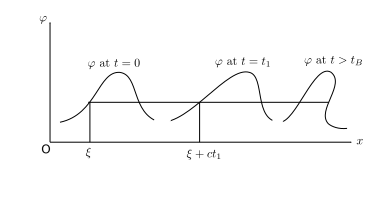
\includegraphics{figures/fig61-1.6.eps}
\caption{}
\label{chap1:fig1.6}
\end{figure}

After some time $t=t_B$, the graph of the curve $\phi$ may become many valued as shown in the above figure \ref{chap1:fig1.6}. This phenomenon is called ``breaking''. It could at least make physical sense in the case of water waves (although the equations are in fact not valid), but in most cases a three valued solution would not make sense. We have to reconsider our approximations and assumptions. 

We\pageoriginale have seen that if $tF'(\xi)+1\neq 0$ then breaking will not occur. A necessary and sufficient condition for breaking to occur is that $F'(\xi)<0$ for some $\xi$. (We assume $c'(\phi)>0)$. For such $\xi'$s the envelope of the characteristics is obtained by eliminating $\xi$ from the equations 
\begin{align*}
x &= \xi + tF(\xi),\\
0 &= tF'(\xi)+1.
\end{align*}

Breaking corresponds to the formation of such an envelope. If we assume that $F'(\xi)$ is minimum only at $\xi_B$ and $F'(\xi_B)<0$, the first breaking time will be 
$$
t_B= -\frac{1}{F'(\xi_B)}=\frac{1}{\left|F'(\xi_B)\right|}.
$$

\begin{figure}[H]
\centering
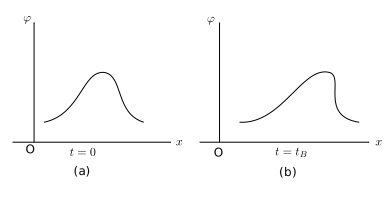
\includegraphics{figures/fig61-1.7.eps}
\caption{}
\label{chap1:fig1.7}
\end{figure}

In the $x,t$, plane the breaking can be seen as follows: since $F'(\xi_B)<0,\, F$ is a decreasing function in a neighbourhood of $\xi_B$ will have increasing slopes and therefore will converge giving a multivalued region. 

\begin{figure}[H]
\centering
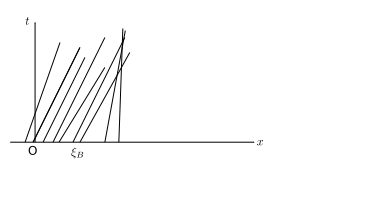
\includegraphics{figures/fig61-1.8.eps}
\caption{}
\label{chap1:fig1.8}
\end{figure}\pageoriginale

From equations
$$
\phi_t= -\frac{F(\xi)f'(\xi)}{tF'(\xi)+1},\phi_x=\frac{f'(\xi)} {tF'(\xi)+1},
$$
we see that $\phi_t,\phi_x$ will become infinite at the time of breaking.

In order to understand the physical meaning of breaking and methods used to correct the solution, we need to look at specific physical problem.

\medskip\noindent
 {\bf \large Probelm on method of characteristics}.

Solve the following:
\begin{enumerate}
\item $\phi_t+e^{-t}\phi_x=0$ in $t>0$, $-\infty < x < \infty$,

$t=0:\phi=\dfrac{1}{1+x^{2}}$

\item $\phi_t+C_0 \phi_x+\alpha\phi=0$ in $t>0$, $-\infty < x < \infty$,

$t=0: \phi =f(x)$

($\alpha$ and $C_0$ positive constants)

\item $x^2 \phi_t+\phi_x+t\phi=0$ in $x>0$, $-\infty < t < \infty$,

$x=0$: $\phi=\Phi (t)$

\item Some\pageoriginale equation as (3), but region $x>0, \, t>0$,

$t=0:\phi=f(x)$, $x>0$,

$x=0:\phi =\Phi(t)$, $t>0$,

\item $\phi_t+\phi\phi_x+\alpha\phi=0$ in $t>0$, $-\infty < x < \infty$,

$t=0:\phi=f(x)$ as shown in Fig. \ref{chap1:fig1.6}.
\end{enumerate}

$\alpha$ is a positive constant.

Show that breaking need not always occur; \ie solution is singlevalued for all $t$ in some cases.
